\documentclass[11pt,a4paper]{article}


\usepackage[utf8]{inputenc}

\usepackage{microtype}
\usepackage[margin=2.4cm]{geometry}
\usepackage{amsmath,amssymb,bm}
\usepackage{graphicx}
\usepackage{booktabs}
\usepackage{xcolor}
\usepackage{tikz}
\usetikzlibrary{arrows.meta,calc,positioning,shapes.geometric,decorations.pathreplacing}
\usepackage{pgfplots}
\pgfplotsset{compat=1.18}
\usepackage{algorithm}
\usepackage{algpseudocode}
\usepackage{caption}
\usepackage{enumitem}
\usepackage{placeins}
\usepackage[colorlinks=true,linkcolor=blue!50!black,citecolor=blue!50!black,urlcolor=blue!50!black]{hyperref}

\captionsetup{font=small,labelfont=bf}
\setlist{itemsep=2pt,topsep=4pt}

% colors of the sketches
\definecolor{cutcol}{RGB}{246,192,150}
\definecolor{candcol}{RGB}{214,228,244}
\definecolor{gridcol}{RGB}{170,170,170}
\definecolor{accent}{RGB}{31,94,168}
\definecolor{ifcol}{RGB}{176,32,32}

\tikzset{
  interface/.style={ifcol, line width=1.2pt},
  signnode/.style={font=\scriptsize, text=black!55, inner sep=0pt},
  sipgface/.style={accent, line width=1.4pt},
  natface/.style={black!70, line width=1.1pt, dash pattern=on 2.5pt off 1.5pt},
}

\newcommand{\T}{\mathcal{T}}
\newcommand{\x}{\bm{x}}
\newcommand{\y}{\bm{y}}
\newcommand{\uu}{\bm{u}}
\newcommand{\nn}{\bm{n}}
\newcommand{\dd}{\,\mathrm{d}}

\algrenewcommand\algorithmicrequire{\textbf{Input:}}
\algrenewcommand\algorithmicensure{\textbf{Output:}}

\title{A narrow-band DG level-set method on cut cells\\[2pt]
\large semi-Lagrangian advection and elliptic reinitialization}
\author{MeltPoolDG \textendash{} application \texttt{mp-narrow-band}}
\date{November 2026}

\begin{document}
\maketitle

\begin{abstract}
\noindent
The level set is represented by discontinuous Galerkin (DG) polynomials only on the cells cut by
the interface. It is advected with a semi-Lagrangian method: the new nodal values are obtained by
tracing the characteristics back to the old cut cells, without any extension of the level set into
neighbor cells. Cells that are not cut store only the sign of the level set. After each step, the
level set is reinitialized on the new cut cells by an elliptic, minimization-based method with a
symmetric interior penalty (SIPG) discretization. This note summarizes the scheme, gives the
algorithms and reports results for a rotating circle and the single-vortex test.
\end{abstract}

\section{Overview}
\label{sec:overview}

The level-set field $\phi$ describes the interface $\Gamma = \{\phi = 0\}$; in this note
$\phi > 0$ inside the bubble. The method keeps three sets of cells of a Cartesian mesh $\T$
(Figure~\ref{fig:sets}):
\begin{itemize}
  \item the \emph{cut cells} $\T^{\Gamma}$, which contain the discrete interface
  $\Gamma_h = \{\phi_h = 0\}$; only these cells carry a polynomial $\phi_h|_K \in Q_p(K)$
  (\texttt{FE\_DGQ}),
  \item the \emph{candidate cells} $\T^{C} \supset \T^{\Gamma}$, the cut cells and the cells sharing
  a vertex with a cut cell; they hold the new level set during one time step,
  \item all other cells, which store only a sign $s_K \in \{-1, +1\}$.
\end{itemize}
A time step consists of three stages: the semi-Lagrangian evaluation of the new level set on the
candidate cells (Section~\ref{sec:sl}), the detection of the new cut cells
(Section~\ref{sec:cutcells}) and the elliptic reinitialization on the new cut cells
(Section~\ref{sec:reinit}). The complete step is given in Section~\ref{sec:step}.

\begin{figure}[ht]
  \centering
  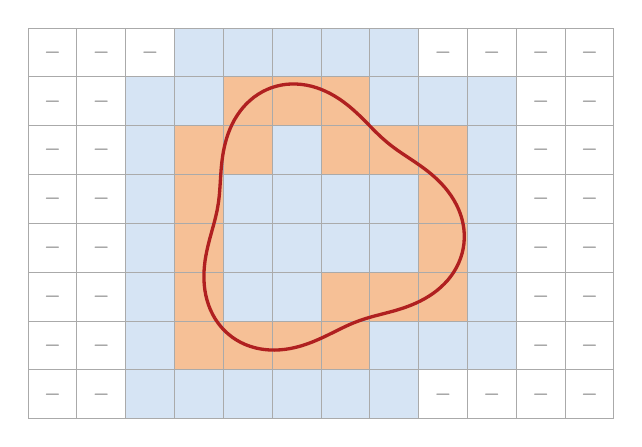
\begin{tikzpicture}[scale=0.62]
\fill[candcol] (2,0) rectangle ++(1,1);
\fill[candcol] (2,1) rectangle ++(1,1);
\fill[candcol] (2,2) rectangle ++(1,1);
\fill[candcol] (2,3) rectangle ++(1,1);
\fill[candcol] (2,4) rectangle ++(1,1);
\fill[candcol] (2,5) rectangle ++(1,1);
\fill[candcol] (2,6) rectangle ++(1,1);
\fill[candcol] (3,0) rectangle ++(1,1);
\fill[candcol] (3,6) rectangle ++(1,1);
\fill[candcol] (3,7) rectangle ++(1,1);
\fill[candcol] (4,0) rectangle ++(1,1);
\fill[candcol] (4,2) rectangle ++(1,1);
\fill[candcol] (4,3) rectangle ++(1,1);
\fill[candcol] (4,4) rectangle ++(1,1);
\fill[candcol] (4,7) rectangle ++(1,1);
\fill[candcol] (5,0) rectangle ++(1,1);
\fill[candcol] (5,2) rectangle ++(1,1);
\fill[candcol] (5,3) rectangle ++(1,1);
\fill[candcol] (5,4) rectangle ++(1,1);
\fill[candcol] (5,5) rectangle ++(1,1);
\fill[candcol] (5,7) rectangle ++(1,1);
\fill[candcol] (6,0) rectangle ++(1,1);
\fill[candcol] (6,3) rectangle ++(1,1);
\fill[candcol] (6,4) rectangle ++(1,1);
\fill[candcol] (6,7) rectangle ++(1,1);
\fill[candcol] (7,0) rectangle ++(1,1);
\fill[candcol] (7,1) rectangle ++(1,1);
\fill[candcol] (7,3) rectangle ++(1,1);
\fill[candcol] (7,4) rectangle ++(1,1);
\fill[candcol] (7,6) rectangle ++(1,1);
\fill[candcol] (7,7) rectangle ++(1,1);
\fill[candcol] (8,1) rectangle ++(1,1);
\fill[candcol] (8,6) rectangle ++(1,1);
\fill[candcol] (9,1) rectangle ++(1,1);
\fill[candcol] (9,2) rectangle ++(1,1);
\fill[candcol] (9,3) rectangle ++(1,1);
\fill[candcol] (9,4) rectangle ++(1,1);
\fill[candcol] (9,5) rectangle ++(1,1);
\fill[candcol] (9,6) rectangle ++(1,1);
\fill[cutcol] (3,1) rectangle ++(1,1);
\fill[cutcol] (3,2) rectangle ++(1,1);
\fill[cutcol] (3,3) rectangle ++(1,1);
\fill[cutcol] (3,4) rectangle ++(1,1);
\fill[cutcol] (3,5) rectangle ++(1,1);
\fill[cutcol] (4,1) rectangle ++(1,1);
\fill[cutcol] (4,5) rectangle ++(1,1);
\fill[cutcol] (4,6) rectangle ++(1,1);
\fill[cutcol] (5,1) rectangle ++(1,1);
\fill[cutcol] (5,6) rectangle ++(1,1);
\fill[cutcol] (6,1) rectangle ++(1,1);
\fill[cutcol] (6,2) rectangle ++(1,1);
\fill[cutcol] (6,5) rectangle ++(1,1);
\fill[cutcol] (6,6) rectangle ++(1,1);
\fill[cutcol] (7,2) rectangle ++(1,1);
\fill[cutcol] (7,5) rectangle ++(1,1);
\fill[cutcol] (8,2) rectangle ++(1,1);
\fill[cutcol] (8,3) rectangle ++(1,1);
\fill[cutcol] (8,4) rectangle ++(1,1);
\fill[cutcol] (8,5) rectangle ++(1,1);
\draw[gridcol, line width=0.3pt] (0,0) grid (12,8);
\node[signnode] at (0.5,0.5) {$-$};
\node[signnode] at (0.5,1.5) {$-$};
\node[signnode] at (0.5,2.5) {$-$};
\node[signnode] at (0.5,3.5) {$-$};
\node[signnode] at (0.5,4.5) {$-$};
\node[signnode] at (0.5,5.5) {$-$};
\node[signnode] at (0.5,6.5) {$-$};
\node[signnode] at (0.5,7.5) {$-$};
\node[signnode] at (1.5,0.5) {$-$};
\node[signnode] at (1.5,1.5) {$-$};
\node[signnode] at (1.5,2.5) {$-$};
\node[signnode] at (1.5,3.5) {$-$};
\node[signnode] at (1.5,4.5) {$-$};
\node[signnode] at (1.5,5.5) {$-$};
\node[signnode] at (1.5,6.5) {$-$};
\node[signnode] at (1.5,7.5) {$-$};
\node[signnode] at (2.5,7.5) {$-$};
\node[signnode] at (8.5,0.5) {$-$};
\node[signnode] at (8.5,7.5) {$-$};
\node[signnode] at (9.5,0.5) {$-$};
\node[signnode] at (9.5,7.5) {$-$};
\node[signnode] at (10.5,0.5) {$-$};
\node[signnode] at (10.5,1.5) {$-$};
\node[signnode] at (10.5,2.5) {$-$};
\node[signnode] at (10.5,3.5) {$-$};
\node[signnode] at (10.5,4.5) {$-$};
\node[signnode] at (10.5,5.5) {$-$};
\node[signnode] at (10.5,6.5) {$-$};
\node[signnode] at (10.5,7.5) {$-$};
\node[signnode] at (11.5,0.5) {$-$};
\node[signnode] at (11.5,1.5) {$-$};
\node[signnode] at (11.5,2.5) {$-$};
\node[signnode] at (11.5,3.5) {$-$};
\node[signnode] at (11.5,4.5) {$-$};
\node[signnode] at (11.5,5.5) {$-$};
\node[signnode] at (11.5,6.5) {$-$};
\node[signnode] at (11.5,7.5) {$-$};
\draw[interface] (8.908,4.000) -- (8.884,4.101) -- (8.853,4.199) -- (8.815,4.296) -- (8.770,4.389) -- (8.720,4.480) -- (8.665,4.566) -- (8.605,4.650) -- (8.542,4.729) -- (8.475,4.804) -- (8.405,4.875) -- (8.334,4.943) -- (8.261,5.007) -- (8.187,5.067) -- (8.113,5.123) -- (8.039,5.177) -- (7.966,5.228) -- (7.894,5.277) -- (7.823,5.324) -- (7.754,5.370) -- (7.687,5.415) -- (7.621,5.460) -- (7.557,5.504) -- (7.496,5.549) -- (7.436,5.594) -- (7.377,5.641) -- (7.320,5.689) -- (7.263,5.739) -- (7.207,5.790) -- (7.152,5.843) -- (7.096,5.898) -- (7.040,5.955) -- (6.982,6.014) -- (6.923,6.074) -- (6.863,6.135) -- (6.800,6.197) -- (6.734,6.259) -- (6.666,6.321) -- (6.594,6.383) -- (6.519,6.443) -- (6.441,6.502) -- (6.359,6.558) -- (6.274,6.611) -- (6.186,6.660) -- (6.094,6.705) -- (6.000,6.746) -- (5.903,6.780) -- (5.804,6.809) -- (5.702,6.831) -- (5.600,6.846) -- (5.497,6.854) -- (5.393,6.855) -- (5.290,6.848) -- (5.188,6.833) -- (5.087,6.810) -- (4.988,6.780) -- (4.892,6.741) -- (4.800,6.696) -- (4.711,6.643) -- (4.626,6.584) -- (4.546,6.518) -- (4.471,6.447) -- (4.401,6.371) -- (4.337,6.290) -- (4.278,6.204) -- (4.224,6.116) -- (4.177,6.025) -- (4.135,5.932) -- (4.098,5.837) -- (4.066,5.741) -- (4.039,5.645) -- (4.017,5.550) -- (3.998,5.455) -- (3.983,5.361) -- (3.971,5.268) -- (3.961,5.177) -- (3.953,5.088) -- (3.947,5.001) -- (3.941,4.917) -- (3.936,4.834) -- (3.931,4.753) -- (3.925,4.674) -- (3.919,4.597) -- (3.911,4.521) -- (3.902,4.446) -- (3.890,4.372) -- (3.878,4.298) -- (3.863,4.225) -- (3.846,4.151) -- (3.828,4.076) -- (3.808,4.000) -- (3.787,3.923) -- (3.765,3.844) -- (3.743,3.763) -- (3.720,3.680) -- (3.698,3.594) -- (3.677,3.506) -- (3.657,3.416) -- (3.639,3.323) -- (3.624,3.228) -- (3.613,3.131) -- (3.605,3.032) -- (3.602,2.932) -- (3.603,2.831) -- (3.610,2.729) -- (3.622,2.627) -- (3.641,2.526) -- (3.666,2.425) -- (3.697,2.327) -- (3.735,2.230) -- (3.780,2.137) -- (3.831,2.047) -- (3.889,1.961) -- (3.953,1.880) -- (4.023,1.804) -- (4.099,1.734) -- (4.180,1.670) -- (4.265,1.613) -- (4.355,1.562) -- (4.449,1.518) -- (4.546,1.482) -- (4.645,1.452) -- (4.746,1.430) -- (4.849,1.415) -- (4.952,1.406) -- (5.055,1.404) -- (5.158,1.409) -- (5.260,1.419) -- (5.360,1.434) -- (5.459,1.455) -- (5.556,1.479) -- (5.650,1.508) -- (5.741,1.539) -- (5.830,1.573) -- (5.916,1.609) -- (6.000,1.646) -- (6.081,1.683) -- (6.159,1.721) -- (6.236,1.759) -- (6.310,1.796) -- (6.382,1.832) -- (6.454,1.866) -- (6.524,1.899) -- (6.593,1.930) -- (6.663,1.960) -- (6.733,1.987) -- (6.803,2.013) -- (6.874,2.037) -- (6.946,2.059) -- (7.020,2.081) -- (7.096,2.102) -- (7.173,2.122) -- (7.253,2.143) -- (7.334,2.164) -- (7.418,2.186) -- (7.503,2.209) -- (7.589,2.235) -- (7.677,2.263) -- (7.767,2.294) -- (7.856,2.329) -- (7.946,2.367) -- (8.035,2.410) -- (8.124,2.457) -- (8.211,2.509) -- (8.296,2.565) -- (8.378,2.627) -- (8.456,2.694) -- (8.531,2.766) -- (8.601,2.842) -- (8.665,2.923) -- (8.724,3.009) -- (8.776,3.098) -- (8.821,3.191) -- (8.859,3.287) -- (8.890,3.386) -- (8.913,3.486) -- (8.928,3.589) -- (8.935,3.692) -- (8.934,3.795) -- (8.925,3.898) -- cycle;
  \end{tikzpicture}
  \hspace{0.6cm}
  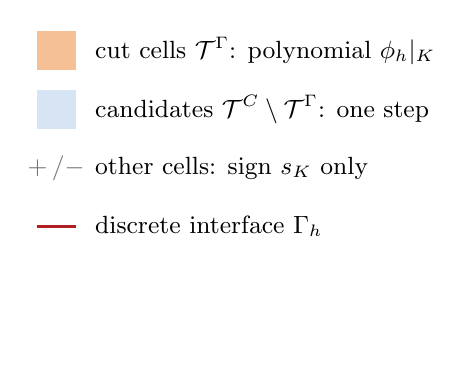
\begin{tikzpicture}[scale=0.62]
    \fill[cutcol] (0,6) rectangle ++(0.8,0.8);
    \node[right] at (1.0,6.4) {\small cut cells $\T^{\Gamma}$: polynomial $\phi_h|_K$};
    \fill[candcol] (0,4.8) rectangle ++(0.8,0.8);
    \node[right] at (1.0,5.2) {\small candidates $\T^{C}\setminus\T^{\Gamma}$: one step};
    \node[signnode, font=\small] at (0.4,4.0) {$+\,/-$};
    \node[right] at (1.0,4.0) {\small other cells: sign $s_K$ only};
    \draw[interface] (0,2.8) -- (0.8,2.8);
    \node[right] at (1.0,2.8) {\small discrete interface $\Gamma_h$};
    \path (0,0) -- (0,1);
  \end{tikzpicture}
  \caption{Cell sets of the semi-Lagrangian narrow band. The level set is stored only on the cut
  cells; the candidate cells (cut cells and their vertex neighbors) receive values only during a
  time step. All other cells know only on which side of the interface they lie.}
  \label{fig:sets}
\end{figure}

\FloatBarrier
\section{Discrete level set on the cut cells}
\label{sec:cutcells}

\paragraph{Cut cells.}
A cell $K$ belongs to $\T^{\Gamma}$ if the zero level set of its polynomial lies inside $K$. This
is decided with the discrete quadrature generator of deal.II (Saye's algorithm for implicitly
defined domains~\cite{Saye2015}): $K$ is cut if the generated surface quadrature for
$\{\phi_h|_K = 0\} \cap K$ is not empty.

\paragraph{Degrees of freedom.}
Two hp-DoFHandlers share the active FE indices. The \emph{cut DoFHandler} holds
\texttt{FE\_DGQ}($p$) on $\T^{\Gamma}$ and \texttt{FE\_Nothing} elsewhere; it stores the level set
between time steps and is used by the reinitialization. The \emph{band DoFHandler} holds
\texttt{FE\_DGQ}($p$) on all candidate cells $\T^{C}$; it receives the semi-Lagrangian values.
Both are rebuilt whenever the cut cells change.

\paragraph{Cell signs.}
A cell that is not cut contains no part of $\Gamma_h$, so $\phi$ has a single sign on it. This sign
can only change if the interface passes through the cell, and the interface can only reach a cell
through the candidate layer. Therefore one integer per cell suffices:
\begin{itemize}
  \item initialization: $s_K = \operatorname{sign} \phi_0(\x_K)$ at the cell center $\x_K$,
  \item update after each step: for every candidate cell that is not cut at $t^{n+1}$, the sign of
  the mean of its $N$ nodal values,
  $s_K = \operatorname{sign}\big(\tfrac{1}{N}\sum_{i} \phi_h^{n+1}(\x_i)\big)$,
  \item the signs of the ghost cells are communicated after each update.
\end{itemize}

\FloatBarrier
\section{Semi-Lagrangian advection}
\label{sec:sl}

The level set satisfies $\partial_t \phi + \uu \cdot \nabla \phi = 0$, i.e., it is constant along
the characteristics $\dot{\bm{X}}(t) = \uu(\bm{X}(t), t)$. The level set at $t^{n+1}$ is therefore
the old level set at the foot points of the characteristics.

\paragraph{Foot points.}
For every node $\x_i$ (support point of \texttt{FE\_DGQ}) of every candidate cell, the
characteristic is integrated backward from $t^{n+1}$ to $t^{n}$ with the classical fourth-order
Runge--Kutta method and the step $-\Delta t$:
\begin{equation}
\begin{aligned}
\bm{k}_1 &= \uu(\x_i, t^{n+1}), &
\bm{k}_2 &= \uu\big(\x_i - \tfrac{\Delta t}{2}\bm{k}_1,\, t^{n+\frac12}\big),\\
\bm{k}_3 &= \uu\big(\x_i - \tfrac{\Delta t}{2}\bm{k}_2,\, t^{n+\frac12}\big), &
\bm{k}_4 &= \uu\big(\x_i - \Delta t\,\bm{k}_3,\, t^{n}\big),
\end{aligned}
\qquad
\x_i^* = \x_i - \frac{\Delta t}{6}\left(\bm{k}_1 + 2\bm{k}_2 + 2\bm{k}_3 + \bm{k}_4\right).
\end{equation}

\paragraph{Old level set at the foot point.}
The new nodal value is the old level set at $\x_i^*$ (Figure~\ref{fig:backtrace}):
\begin{equation}
\label{eq:sl}
\phi_h^{n+1}(\x_i) =
\begin{cases}
\phi_h^{n}|_K(\x_i^*), & \x_i^* \in K \in \T^{\Gamma,n} \quad \text{(cut cell)},\\[3pt]
s_K\, |\nabla \phi_h^n(\y)|\, d(\x_i^*, \y), & \x_i^* \in K \notin \T^{\Gamma,n} \quad
\text{(not cut)}.
\end{cases}
\end{equation}
In the second case, $\y$ is the closest point of $\x_i^*$ on the old discrete interface
$\Gamma_h^n$. It is computed per candidate cut cell by Newton's method for the optimality conditions
of $\min_{\y} \tfrac12|\x_i^* - \y|^2$ subject to $\phi_h(\y) = 0$ (Saye~\cite{Saye2014}),
\begin{equation}
\y - \x_i^* + \lambda \nabla\phi_h(\y) = \bm{0}, \qquad \phi_h(\y) = 0,
\end{equation}
starting from the nearest quadrature point of $\Gamma_h^n$. The candidate cut cells are those of the
nearest quadrature points of the interface (8 in 2D); the one with the smallest distance estimate
\begin{equation}
d(\x_i^*, \y) = |\x_i^* - \y| + \frac{|\phi_h(\y)|}{|\nabla \phi_h(\y)|}
\end{equation}
is taken. For a converged closest point, $s_K |\nabla\phi_h(\y)|\, d$ equals the first-order Taylor
value $\phi_h(\y) + \nabla\phi_h(\y)\cdot(\x_i^* - \y)$. At an open end of $\Gamma_h^n$, the Taylor
value would vanish on the continuation of the tangent, while the distance to the end point does not.

\begin{figure}[ht]
  \centering
  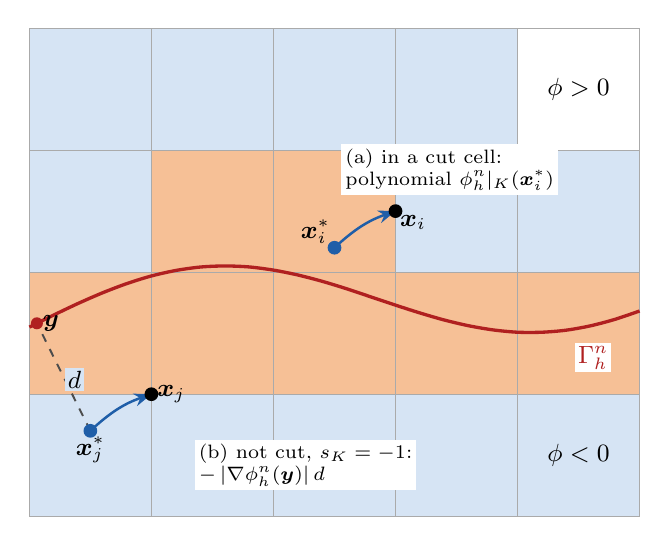
\begin{tikzpicture}[scale=1.55]
    % cells: cut cells and candidates of the zoom
    \foreach \c in {(0,1),(1,1),(1,2),(2,1),(2,2),(3,1),(4,1)} {\fill[cutcol] \c rectangle ++(1,1);}
    \foreach \c in {(0,0),(1,0),(2,0),(3,0),(4,0),(0,2),(3,2),(4,2),(0,3),(1,3),(2,3),(3,3)}
      {\fill[candcol] \c rectangle ++(1,1);}
    \draw[gridcol, line width=0.3pt] (0,0) grid (5,4);
    \draw[interface] plot[smooth] coordinates {(0.000,1.550) (0.200,1.649) (0.400,1.744) (0.600,1.831)
      (0.800,1.907) (1.000,1.969) (1.200,2.014) (1.400,2.042) (1.600,2.051) (1.800,2.043) (2.000,2.017)
      (2.200,1.977) (2.400,1.925) (2.600,1.864) (2.800,1.797) (3.000,1.730) (3.200,1.666) (3.400,1.608)
      (3.600,1.561) (3.800,1.527) (4.000,1.508) (4.200,1.508) (4.400,1.525) (4.600,1.561) (4.800,1.614)
      (5.000,1.682)};
    \node[ifcol, font=\small, fill=white, inner sep=1pt] at (4.62,1.3) {$\Gamma_h^n$};
    \node[font=\small] at (4.5,3.5) {$\phi > 0$};
    \node[font=\small] at (4.5,0.5) {$\phi < 0$};
    % case (a): foot point in a cut cell
    \coordinate (A) at (3.0,2.5);
    \coordinate (As) at (2.5,2.2);
    \draw[-{Stealth[length=2.2mm]}, accent, line width=0.9pt] (As) to[bend left=12] (A);
    \fill[black] (A) circle (1.6pt);
    \fill[accent] (As) circle (1.6pt);
    \node[below right, font=\small, inner sep=1.5pt] at (A) {$\x_i$};
    \node[above left, font=\small, inner sep=1.5pt] at (As) {$\x_i^*$};
    \node[font=\scriptsize, align=left, anchor=west, fill=white, inner sep=1.5pt] at (2.55,2.84)
      {(a) in a cut cell:\\ polynomial $\phi_h^n|_K(\x_i^*)$};
    % case (b): foot point in a cell that is not cut
    \coordinate (B) at (1.0,1.0);
    \coordinate (Bs) at (0.5,0.7);
    \coordinate (Y) at (0.062,1.581);
    \draw[-{Stealth[length=2.2mm]}, accent, line width=0.9pt] (Bs) to[bend left=12] (B);
    \draw[black!70, dashed, line width=0.7pt] (Bs) -- (Y);
    \fill[black] (B) circle (1.6pt);
    \fill[accent] (Bs) circle (1.6pt);
    \fill[ifcol] (Y) circle (1.4pt);
    \node[right, font=\small, inner sep=2pt] at (B) {$\x_j$};
    \node[below, font=\small, inner sep=2pt] at (Bs) {$\x_j^*$};
    \node[right, font=\small, inner sep=2pt] at (Y) {$\y$};
    \node[font=\small, fill=candcol, inner sep=1pt] at (0.37,1.12) {$d$};
    \node[font=\scriptsize, align=left, anchor=west, fill=white, inner sep=1.5pt] at (1.35,0.42)
      {(b) not cut, $s_K = -1$:\\ $-\,|\nabla\phi_h^n(\y)|\,d$};
  \end{tikzpicture}
  \caption{Back-tracing of two nodes of candidate cells (orange: cut cells, blue: candidate cells
  that are not cut). The arrows are the characteristics from the foot point to the node over one
  time step. (a)~The foot point lies in a cut cell: its polynomial is evaluated. (b)~The foot point
  lies in a cell that is not cut: the scaled distance to the old interface with the stored sign of
  that cell.}
  \label{fig:backtrace}
\end{figure}

\paragraph{Nodal interpolation and new cut cells.}
The values \eqref{eq:sl} are the nodal values of $\phi_h^{n+1}$ on the band DoFHandler. The new cut
cells $\T^{\Gamma,n+1} \subseteq \T^{C}$ are those candidate cells in which $\phi_h^{n+1}$ has a zero
(Section~\ref{sec:cutcells}). Their polynomials are copied to the new cut DoFHandler; the values of
the other candidate cells are only used to update the signs and are then discarded.

\paragraph{Properties.}
\begin{itemize}
  \item \emph{No extrapolation.} The interface at $t^{n+1}$ can only come from material that was in
  a cut cell at $t^{n}$. A node whose foot point lies in a cell that is not cut always gets the sign
  of that cell, so no new interface appears there, and an open end of $\Gamma_h$ (an under-resolved
  tail) moves with the flow instead of being prolonged.
  \item \emph{Time step.} There is no stability limit of an explicit DG scheme. The foot points must
  lie in the candidate cell or its vertex neighbors, i.e., the displacement $|\x_i - \x_i^*|$ must
  stay below one cell. The maximum displacement relative to the cell size is printed in each step.
  \item \emph{Accuracy.} Every step adds an interpolation error of order $h^{p+1}$, so the error
  after $T/\Delta t$ steps behaves like $h^{p+1}/\Delta t$, i.e., like $h^{p}$ for a fixed ratio
  $\Delta t / h$. Large time steps (displacement of about $0.3h$ to $0.7h$) are more accurate than
  small ones.
  \item \emph{Conservation.} The method is not conservative.
\end{itemize}

\begin{algorithm}[ht]
  \caption{Semi-Lagrangian evaluation of $\phi_h^{n+1}$ on the candidate cells}
  \label{alg:sl}
  \begin{algorithmic}[1]
    \Require $\phi_h^n$ on $\T^{\Gamma,n}$, signs $s_K$, velocity $\uu$, $t^n$, $\Delta t$
    \Ensure nodal values of $\phi_h^{n+1}$ on $\T^{C} = \T^{\Gamma,n} \cup \{$vertex neighbors$\}$
    \State gather the cut cells of all processes: affine map, DoF values, quadrature points of
    $\Gamma_h^n$
    \State build search trees of the cut-cell bounding boxes and of the interface quadrature points
    \For{each locally owned cell $C \in \T^{C}$}
      \For{each node $\x_i$ of $C$}
        \State $\x_i^* \gets$ RK4 backward along $\uu$ from $t^{n+1}$ to $t^n$
        \If{$\x_i^* \in K$ for a cut cell $K$ (box tree, then reference coordinates)}
          \State $\phi_h^{n+1}(\x_i) \gets \phi_h^n|_K(\x_i^*)$
        \Else
          \State $\y \gets$ closest point on $\Gamma_h^n$ (Newton in the cut cells of the nearest
          interface points)
          \State $K \gets$ cell containing $\x_i^*$ among $C$ and its vertex neighbors
          \If{$K$ found}
            \State $\phi_h^{n+1}(\x_i) \gets s_K\, |\nabla\phi_h^n(\y)|\, d(\x_i^*, \y)$
          \Else
            \State $\phi_h^{n+1}(\x_i) \gets \operatorname{sign}\!\big(\phi_h^n(\y) +
            \nabla\phi_h^n(\y)\cdot(\x_i^*-\y)\big)\, |\nabla\phi_h^n(\y)|\, d(\x_i^*, \y)$
            \Comment{reported}
          \EndIf
        \EndIf
      \EndFor
    \EndFor
  \end{algorithmic}
\end{algorithm}

\section{Elliptic reinitialization on the cut cells}
\label{sec:reinit}

The advected level set loses the signed-distance property. It is restored on the cut cells only,
while the position of the interface is kept. Following Basting and Kuzmin~\cite{BastingKuzmin2013}
and Adams et al.~\cite{Adams2019}, the reinitialized level set minimizes
\begin{equation}
\int_{\Omega_\Gamma} \big(|\nabla\phi| - 1\big)^2 \dd x
+ \frac{\gamma}{2} \int_{\Gamma} \phi^2 \dd s,
\end{equation}
where $\Omega_\Gamma = \bigcup_{K \in \T^{\Gamma}} K$ is the union of the cut cells and $\Gamma$ is
the zero level set before the reinitialization; the second term enforces the interface position
weakly. The nonlinear problem is solved by the fixed-point iteration: find $\phi^{k+1}$ with
\begin{equation}
a(\phi^{k+1}, v) = l(\phi^k; v) \quad \text{for all } v \in Q_p(\T^{\Gamma}),
\end{equation}
with the SIPG bilinear form on the faces $\mathcal{F}_\Gamma$ between two cut cells
\begin{equation}
a(\phi, v) = (\nabla\phi, \nabla v)_{\Omega_\Gamma}
- (\{\nabla\phi\}\cdot\nn, [v])_{\mathcal{F}_\Gamma}
- ([\phi], \{\nabla v\}\cdot\nn)_{\mathcal{F}_\Gamma}
+ \sigma ([\phi], [v])_{\mathcal{F}_\Gamma}
+ \gamma (\phi, v)_{\Gamma},
\end{equation}
the linear form
\begin{equation}
l(\phi^k; v) = \big(g(|\nabla\phi^k|)\nabla\phi^k, \nabla v\big)_{\Omega_\Gamma}
- \big(\{g(|\nabla\phi^k|)\nabla\phi^k\}\cdot\nn, [v]\big)_{\mathcal{F}_\Gamma},
\qquad
g(s) = \begin{cases} 1/s, & s > 1,\\ 2 - s, & s \le 1,\end{cases}
\end{equation}
and the interior penalty $\sigma = c_{\mathrm{ip}}\, p^3 / h_{\min}$ (default $c_{\mathrm{ip}} = 10$).
The faces between a cut cell and a cell that is not cut, and the domain boundary, are part of the
boundary of $\Omega_\Gamma$, where the natural boundary condition of the minimization problem holds;
no face integrals are evaluated there (Figure~\ref{fig:reinit}). Only the cells and faces of
$\Omega_\Gamma$ are visited, so the cost scales with the size of the interface. The linear systems
are solved matrix-free with CG.

The reinitialization is triggered every $f$-th step (parameter \texttt{reinitialization frequency})
or when the eikonal error on the cut cells,
$\big(\int_{\Omega_\Gamma}(|\nabla\phi_h|-1)^2\dd x / |\Omega_\Gamma|\big)^{1/2}$, exceeds a
threshold (\texttt{reinitialization eikonal threshold}).

\begin{figure}[ht]
  \centering
  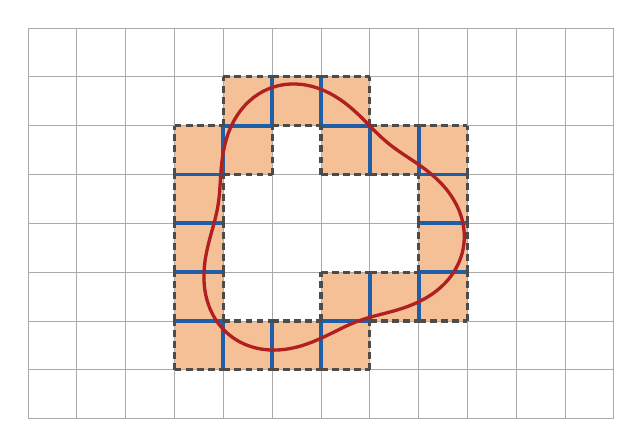
\begin{tikzpicture}[scale=0.62]
\fill[cutcol] (3,1) rectangle ++(1,1);
\fill[cutcol] (3,2) rectangle ++(1,1);
\fill[cutcol] (3,3) rectangle ++(1,1);
\fill[cutcol] (3,4) rectangle ++(1,1);
\fill[cutcol] (3,5) rectangle ++(1,1);
\fill[cutcol] (4,1) rectangle ++(1,1);
\fill[cutcol] (4,5) rectangle ++(1,1);
\fill[cutcol] (4,6) rectangle ++(1,1);
\fill[cutcol] (5,1) rectangle ++(1,1);
\fill[cutcol] (5,6) rectangle ++(1,1);
\fill[cutcol] (6,1) rectangle ++(1,1);
\fill[cutcol] (6,2) rectangle ++(1,1);
\fill[cutcol] (6,5) rectangle ++(1,1);
\fill[cutcol] (6,6) rectangle ++(1,1);
\fill[cutcol] (7,2) rectangle ++(1,1);
\fill[cutcol] (7,5) rectangle ++(1,1);
\fill[cutcol] (8,2) rectangle ++(1,1);
\fill[cutcol] (8,3) rectangle ++(1,1);
\fill[cutcol] (8,4) rectangle ++(1,1);
\fill[cutcol] (8,5) rectangle ++(1,1);
\draw[gridcol, line width=0.3pt] (0,0) grid (12,8);
\draw[sipgface] (4,1) -- (4,2) (4,5) -- (4,6) (5,1) -- (5,2) (5,6) -- (5,7) (6,1) -- (6,2) (6,6) -- (6,7) (7,2) -- (7,3) (7,5) -- (7,6) (8,2) -- (8,3) (8,5) -- (8,6) (3,2) -- (4,2) (3,3) -- (4,3) (3,4) -- (4,4) (3,5) -- (4,5) (4,6) -- (5,6) (6,2) -- (7,2) (6,6) -- (7,6) (8,3) -- (9,3) (8,4) -- (9,4) (8,5) -- (9,5);
\draw[natface] (3,1) -- (3,2) (3,2) -- (3,3) (3,3) -- (3,4) (3,4) -- (3,5) (3,5) -- (3,6) (4,2) -- (4,3) (4,3) -- (4,4) (4,4) -- (4,5) (4,6) -- (4,7) (5,5) -- (5,6) (6,2) -- (6,3) (6,5) -- (6,6) (7,1) -- (7,2) (7,6) -- (7,7) (8,3) -- (8,4) (8,4) -- (8,5) (9,2) -- (9,3) (9,3) -- (9,4) (9,4) -- (9,5) (9,5) -- (9,6) (3,1) -- (4,1) (3,6) -- (4,6) (4,1) -- (5,1) (4,2) -- (5,2) (4,5) -- (5,5) (4,7) -- (5,7) (5,1) -- (6,1) (5,2) -- (6,2) (5,6) -- (6,6) (5,7) -- (6,7) (6,1) -- (7,1) (6,3) -- (7,3) (6,5) -- (7,5) (6,7) -- (7,7) (7,2) -- (8,2) (7,3) -- (8,3) (7,5) -- (8,5) (7,6) -- (8,6) (8,2) -- (9,2) (8,6) -- (9,6);
\draw[interface] (8.908,4.000) -- (8.884,4.101) -- (8.853,4.199) -- (8.815,4.296) -- (8.770,4.389) -- (8.720,4.480) -- (8.665,4.566) -- (8.605,4.650) -- (8.542,4.729) -- (8.475,4.804) -- (8.405,4.875) -- (8.334,4.943) -- (8.261,5.007) -- (8.187,5.067) -- (8.113,5.123) -- (8.039,5.177) -- (7.966,5.228) -- (7.894,5.277) -- (7.823,5.324) -- (7.754,5.370) -- (7.687,5.415) -- (7.621,5.460) -- (7.557,5.504) -- (7.496,5.549) -- (7.436,5.594) -- (7.377,5.641) -- (7.320,5.689) -- (7.263,5.739) -- (7.207,5.790) -- (7.152,5.843) -- (7.096,5.898) -- (7.040,5.955) -- (6.982,6.014) -- (6.923,6.074) -- (6.863,6.135) -- (6.800,6.197) -- (6.734,6.259) -- (6.666,6.321) -- (6.594,6.383) -- (6.519,6.443) -- (6.441,6.502) -- (6.359,6.558) -- (6.274,6.611) -- (6.186,6.660) -- (6.094,6.705) -- (6.000,6.746) -- (5.903,6.780) -- (5.804,6.809) -- (5.702,6.831) -- (5.600,6.846) -- (5.497,6.854) -- (5.393,6.855) -- (5.290,6.848) -- (5.188,6.833) -- (5.087,6.810) -- (4.988,6.780) -- (4.892,6.741) -- (4.800,6.696) -- (4.711,6.643) -- (4.626,6.584) -- (4.546,6.518) -- (4.471,6.447) -- (4.401,6.371) -- (4.337,6.290) -- (4.278,6.204) -- (4.224,6.116) -- (4.177,6.025) -- (4.135,5.932) -- (4.098,5.837) -- (4.066,5.741) -- (4.039,5.645) -- (4.017,5.550) -- (3.998,5.455) -- (3.983,5.361) -- (3.971,5.268) -- (3.961,5.177) -- (3.953,5.088) -- (3.947,5.001) -- (3.941,4.917) -- (3.936,4.834) -- (3.931,4.753) -- (3.925,4.674) -- (3.919,4.597) -- (3.911,4.521) -- (3.902,4.446) -- (3.890,4.372) -- (3.878,4.298) -- (3.863,4.225) -- (3.846,4.151) -- (3.828,4.076) -- (3.808,4.000) -- (3.787,3.923) -- (3.765,3.844) -- (3.743,3.763) -- (3.720,3.680) -- (3.698,3.594) -- (3.677,3.506) -- (3.657,3.416) -- (3.639,3.323) -- (3.624,3.228) -- (3.613,3.131) -- (3.605,3.032) -- (3.602,2.932) -- (3.603,2.831) -- (3.610,2.729) -- (3.622,2.627) -- (3.641,2.526) -- (3.666,2.425) -- (3.697,2.327) -- (3.735,2.230) -- (3.780,2.137) -- (3.831,2.047) -- (3.889,1.961) -- (3.953,1.880) -- (4.023,1.804) -- (4.099,1.734) -- (4.180,1.670) -- (4.265,1.613) -- (4.355,1.562) -- (4.449,1.518) -- (4.546,1.482) -- (4.645,1.452) -- (4.746,1.430) -- (4.849,1.415) -- (4.952,1.406) -- (5.055,1.404) -- (5.158,1.409) -- (5.260,1.419) -- (5.360,1.434) -- (5.459,1.455) -- (5.556,1.479) -- (5.650,1.508) -- (5.741,1.539) -- (5.830,1.573) -- (5.916,1.609) -- (6.000,1.646) -- (6.081,1.683) -- (6.159,1.721) -- (6.236,1.759) -- (6.310,1.796) -- (6.382,1.832) -- (6.454,1.866) -- (6.524,1.899) -- (6.593,1.930) -- (6.663,1.960) -- (6.733,1.987) -- (6.803,2.013) -- (6.874,2.037) -- (6.946,2.059) -- (7.020,2.081) -- (7.096,2.102) -- (7.173,2.122) -- (7.253,2.143) -- (7.334,2.164) -- (7.418,2.186) -- (7.503,2.209) -- (7.589,2.235) -- (7.677,2.263) -- (7.767,2.294) -- (7.856,2.329) -- (7.946,2.367) -- (8.035,2.410) -- (8.124,2.457) -- (8.211,2.509) -- (8.296,2.565) -- (8.378,2.627) -- (8.456,2.694) -- (8.531,2.766) -- (8.601,2.842) -- (8.665,2.923) -- (8.724,3.009) -- (8.776,3.098) -- (8.821,3.191) -- (8.859,3.287) -- (8.890,3.386) -- (8.913,3.486) -- (8.928,3.589) -- (8.935,3.692) -- (8.934,3.795) -- (8.925,3.898) -- cycle;
  \end{tikzpicture}
  \hspace{0.6cm}
  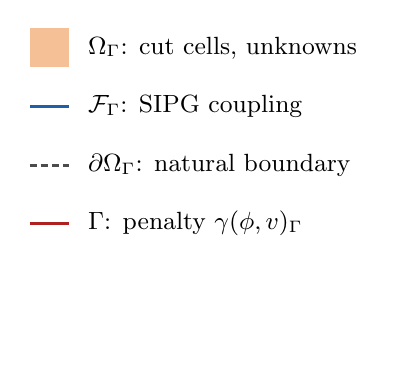
\begin{tikzpicture}[scale=0.62]
    \fill[cutcol] (0,6) rectangle ++(0.8,0.8);
    \node[right] at (1.0,6.4) {\small $\Omega_\Gamma$: cut cells, unknowns};
    \draw[sipgface] (0,5.2) -- (0.8,5.2);
    \node[right] at (1.0,5.2) {\small $\mathcal{F}_\Gamma$: SIPG coupling};
    \draw[natface] (0,4.0) -- (0.8,4.0);
    \node[right] at (1.0,4.0) {\small $\partial\Omega_\Gamma$: natural boundary};
    \draw[interface] (0,2.8) -- (0.8,2.8);
    \node[right] at (1.0,2.8) {\small $\Gamma$: penalty $\gamma(\phi, v)_\Gamma$};
    \path (0,0) -- (0,1);
  \end{tikzpicture}
  \caption{Domain of the elliptic reinitialization: only the cut cells carry unknowns. The cut cells
  are coupled by SIPG terms across their common faces; at the faces to cells that are not cut, the
  natural boundary condition applies. The interface position is enforced by a penalty on $\Gamma$.}
  \label{fig:reinit}
\end{figure}

\begin{algorithm}[ht]
  \caption{Elliptic reinitialization on the cut cells}
  \label{alg:reinit}
  \begin{algorithmic}[1]
    \Require $\phi_h$ on $\T^{\Gamma}$
    \Ensure reinitialized $\phi_h$ on $\T^{\Gamma}$, same zero level set (weakly)
    \State $\Gamma \gets \{\phi_h = 0\}$; surface quadrature on the cut cells
    \State $\phi^0 \gets \phi_h$, \quad $k \gets 0$
    \Repeat
      \State assemble $l(\phi^k; \cdot)$ on $\Omega_\Gamma$ and $\mathcal{F}_\Gamma$
      \State solve $a(\phi^{k+1}, v) = l(\phi^k; v)$ for all $v$ \Comment{matrix-free CG}
      \State $k \gets k + 1$
    \Until{residual $< 10^{-5}$ and $\|\phi^{k} - \phi^{k-1}\| < 10^{-5}$}
    \State $\phi_h \gets \phi^{k}$
  \end{algorithmic}
\end{algorithm}

\FloatBarrier
\section{The complete time step}
\label{sec:step}

The reinitialization is the last stage of a time step. It acts on the cut cells found from the
advected level set, and the next semi-Lagrangian step traces back into exactly these reinitialized
polynomials. The signs need no reinitialization: they only state on which side a cell lies, and the
reinitialization keeps the interface in place. Figure~\ref{fig:flow} shows the flow of one step and
Algorithm~\ref{alg:step} the complete method.

\begin{figure}[tbp]
  \centering
  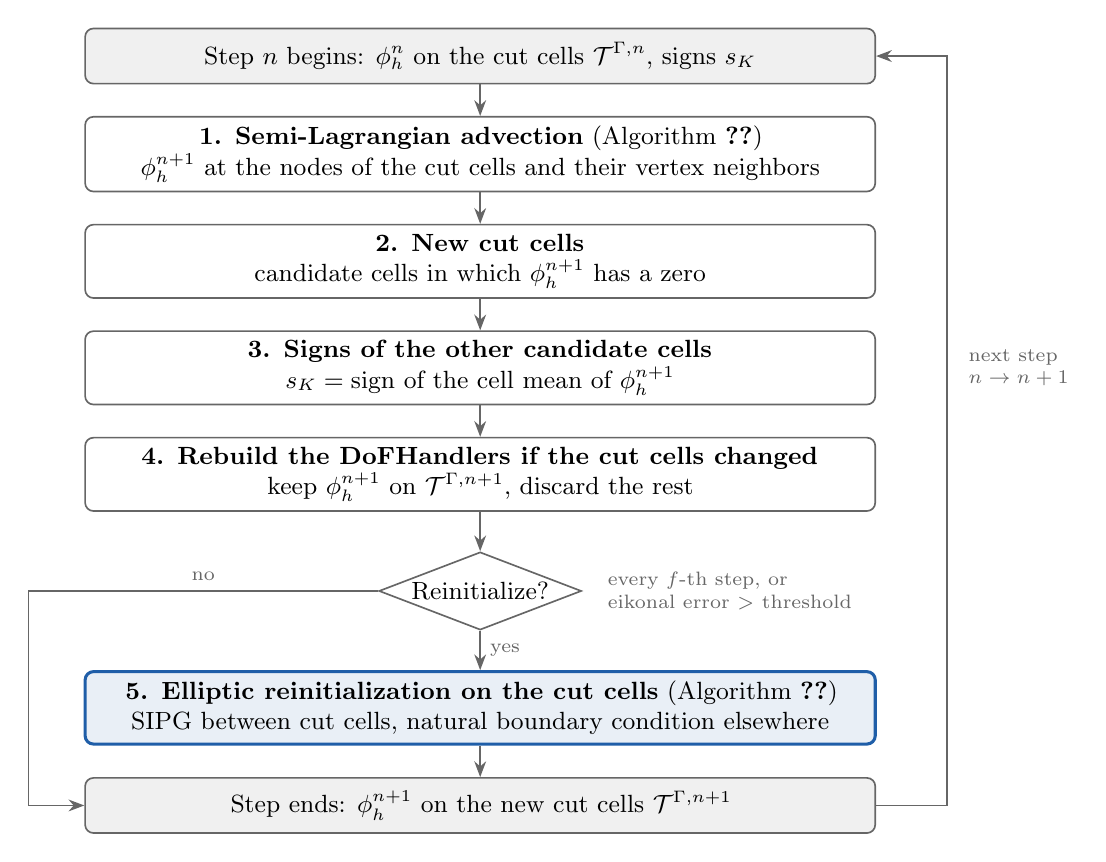
\begin{tikzpicture}[
      node distance=4mm,
      box/.style={draw=black!60, rounded corners=3pt, align=flush center, text width=9.8cm,
        minimum height=7mm, font=\small, line width=0.6pt},
      io/.style={box, fill=black!6},
      hl/.style={box, draw=accent, fill=accent!10, line width=1.1pt},
      dec/.style={diamond, draw=black!60, aspect=2.6, inner sep=1pt, font=\small, line width=0.6pt},
      arr/.style={-{Stealth[length=2mm]}, black!60, line width=0.6pt},
      lab/.style={font=\scriptsize, text=black!60}]
    \node[io] (start) {Step $n$ begins: $\phi_h^n$ on the cut cells $\T^{\Gamma,n}$, signs $s_K$};
    \node[box, below=of start] (sl) {\textbf{1. Semi-Lagrangian advection} (Algorithm~\ref{alg:sl})\\
      $\phi_h^{n+1}$ at the nodes of the cut cells and their vertex neighbors};
    \node[box, below=of sl] (cut) {\textbf{2. New cut cells}\\
      candidate cells in which $\phi_h^{n+1}$ has a zero};
    \node[box, below=of cut] (sign) {\textbf{3. Signs of the other candidate cells}\\
      $s_K = \operatorname{sign}$ of the cell mean of $\phi_h^{n+1}$};
    \node[box, below=of sign] (band) {\textbf{4. Rebuild the DoFHandlers if the cut cells changed}\\
      keep $\phi_h^{n+1}$ on $\T^{\Gamma,n+1}$, discard the rest};
    \node[dec, below=5mm of band] (dec) {Reinitialize?};
    \node[hl, below=5mm of dec] (reinit) {\textbf{5. Elliptic reinitialization on the cut cells}
      (Algorithm~\ref{alg:reinit})\\ SIPG between cut cells, natural boundary condition elsewhere};
    \node[io, below=of reinit] (end) {Step ends: $\phi_h^{n+1}$ on the new cut cells $\T^{\Gamma,n+1}$};
    \coordinate (L) at ($(reinit.west)+(-0.7,0)$);
    \coordinate (R) at ($(start.east)+(0.9,0)$);
    \draw[arr] (start) -- (sl);
    \draw[arr] (sl) -- (cut);
    \draw[arr] (cut) -- (sign);
    \draw[arr] (sign) -- (band);
    \draw[arr] (band) -- (dec);
    \draw[arr] (dec) -- node[lab, right] {yes} (reinit);
    \draw[arr] (reinit) -- (end);
    \draw[arr] (dec.west) -- node[lab, above, pos=0.5] {no} (dec.west -| L) |- (end.west);
    \draw[arr] (end.east) -- (end.east -| R) |- (start.east);
    \node[lab, align=left, anchor=west] at ($(R |- sign)+(0.15,0)$) {next step\\ $n \to n+1$};
    \node[lab, right=2mm of dec, align=left] {every $f$-th step, or\\ eikonal error $>$ threshold};
  \end{tikzpicture}
  \caption{One time step of the semi-Lagrangian narrow band. The reinitialization closes the step
  and acts on the new cut cells only.}
  \label{fig:flow}
\end{figure}

\begin{algorithm}[tbp]
  \caption{Semi-Lagrangian narrow-band level set}
  \label{alg:step}
  \begin{algorithmic}[1]
    \Require initial level set $\phi_0$, velocity $\uu$, $\Delta t$, reinitialization frequency $f$
    \Statex \textit{Initialization}
    \State $\T^{\Gamma} \gets$ cells intersected by $\phi_0$ (mesh classifier, then the discrete
    check of Section~\ref{sec:cutcells})
    \State $\phi_h \gets$ interpolation of $\phi_0$ on $\T^{\Gamma}$; \quad
    $s_K \gets \operatorname{sign}\phi_0(\x_K)$ for all cells
    \State optionally $\phi_h \gets$ \Call{Reinitialize}{$\phi_h$, $\T^{\Gamma}$}
    \Statex \textit{Time loop}
    \For{$n = 0, 1, \dots$}
      \State $\T^{C} \gets \T^{\Gamma} \cup \{K : K \text{ shares a vertex with a cut cell}\}$
      \State $\phi_h^{n+1} \gets$ semi-Lagrangian evaluation on $\T^{C}$ (Algorithm~\ref{alg:sl})
      \State $\T^{\Gamma,n+1} \gets \{K \in \T^{C} : \phi_h^{n+1}|_K \text{ has a zero in } K\}$
      \For{$K \in \T^{C} \setminus \T^{\Gamma,n+1}$}
        \State $s_K \gets \operatorname{sign}$ of the mean of the nodal values of
        $\phi_h^{n+1}|_K$
      \EndFor
      \State exchange $s_K$ with the ghost cells
      \If{$\T^{\Gamma,n+1} \neq \T^{\Gamma}$}
        \State rebuild the cut and band DoFHandlers
      \EndIf
      \State $\phi_h \gets \phi_h^{n+1}|_{\T^{\Gamma,n+1}}$; \quad $\T^{\Gamma} \gets \T^{\Gamma,n+1}$
      \If{$(n+1) \bmod f = 0$ \textbf{or} eikonal error $>$ threshold}
        \State $\phi_h \gets$ \Call{Reinitialize}{$\phi_h$, $\T^{\Gamma}$}
        \Comment{Algorithm~\ref{alg:reinit}}
      \EndIf
    \EndFor
  \end{algorithmic}
\end{algorithm}

\section{Comparison with the DG band advection}
\label{sec:band}

The alternative in \texttt{mp-narrow-band} (\texttt{narrow band/type = extension}) advects the level
set with an upwind DG scheme in non-conservative form on a band of the cut cells and their face
neighbors $\T^{B}$: find $\phi_h \in Q_p(\T^{B})$ with
\begin{equation}
\sum_{K \in \T^{B}} \Big[ (\partial_t \phi_h + \uu\cdot\nabla\phi_h, v)_K
- \int_{\partial K^-} (\uu\cdot\nn_K)\,(\phi_h^{\mathrm{int}} - \phi_h^{\mathrm{ext}})\, v \dd s
\Big] = 0,
\end{equation}
with the inflow boundary $\partial K^-$ and $\phi_h^{\mathrm{ext}} = \phi_h^{\mathrm{int}}$ at the
outer boundary of the band, integrated with a third-order SSP Runge--Kutta method. Before each step,
the level set of the neighbor cells is reconstructed by an extension from the cut cells
(ghost-penalty or closest-point extension). The reinitialization is the same as in
Section~\ref{sec:reinit}.

\begin{table}[ht]
  \centering
  \small
  \caption{DG band advection and semi-Lagrangian narrow band.}
  \label{tab:compare}
  \begin{tabular}{@{}p{3.3cm}p{5.6cm}p{5.6cm}@{}}
    \toprule
    & DG band (\texttt{extension}) & semi-Lagrangian (\texttt{semi\_lagrangian}) \\
    \midrule
    Stored level set & cut cells and face neighbors & cut cells only (plus one sign per cell) \\
    Data outside the cut cells & polynomial extension in every step & none; distance with the sign of
    the cell \\
    Time step & explicit DG limit, CFL $\sim 1/(2p+1)$ & displacement below one cell \\
    Order (resolved) & $p+1$ (observed 2.2--2.6 for $p=2$) & $p$ (observed 1.9 for $p=2$) \\
    Under-resolved tails & extrapolation prolongs open ends, spurious interfaces & tail breaks up,
    no spurious interfaces \\
    Extra cost & extension (global linear solve on the band) & closest-point search per node
    outside the cut cells \\
    \bottomrule
  \end{tabular}
\end{table}

\FloatBarrier
\section{Results}
\label{sec:results}

All results use $p = 2$, the elliptic reinitialization on the cut cells with the interface penalty
$\gamma = 10^4$, and the interface error
$e_\Gamma = \big(\int_{\Gamma_h} d_{\mathrm{ex}}^2 \dd s / |\Gamma_h|\big)^{1/2}$ with the exact
signed distance $d_{\mathrm{ex}}$ at the final time.

\paragraph{Rotating circle.}
A circle of radius $0.25$ centered at $(0, 0.5)$ rotates once about the origin in
$\Omega = [-1, 1]^2$ (angular velocity $2\pi$, $t \in [0, 1]$). Table~\ref{tab:rc} and
Figure~\ref{fig:rc} compare the DG band advection (ghost-penalty extension, reinitialization every
10 steps) with the semi-Lagrangian method at the same and at a four times larger time step.

\begin{table}[ht]
  \centering
  \small
  \caption{Rotating circle, interface error $e_\Gamma$ after one revolution (EOC: experimental order
  of convergence). DG band and SL with $\Delta t$: $\Delta t = 0.004, 0.002, 0.001$, reinitialization
  every 10 steps. SL with $4\Delta t$: reinitialization every 3, 3, 2 steps.}
  \label{tab:rc}
  \begin{tabular}{@{}ccrrrrrr@{}}
    \toprule
    cells & $h$ & \multicolumn{2}{c}{DG band, $\Delta t$} & \multicolumn{2}{c}{SL, $\Delta t$}
      & \multicolumn{2}{c}{SL, $4\Delta t$} \\
    \cmidrule(lr){3-4}\cmidrule(lr){5-6}\cmidrule(l){7-8}
    & & $e_\Gamma$ & EOC & $e_\Gamma$ & EOC & $e_\Gamma$ & EOC \\
    \midrule
    $16^2$ & $0.125$  & $1.32\cdot10^{-3}$ & --   & $7.88\cdot10^{-3}$ & --   & $3.30\cdot10^{-3}$ & -- \\
    $32^2$ & $0.0625$ & $2.17\cdot10^{-4}$ & 2.61 & $2.19\cdot10^{-3}$ & 1.85 & $8.90\cdot10^{-4}$ & 1.89 \\
    $64^2$ & $0.03125$& $4.86\cdot10^{-5}$ & 2.16 & $5.53\cdot10^{-4}$ & 1.98 & $2.38\cdot10^{-4}$ & 1.91 \\
    \bottomrule
  \end{tabular}
\end{table}

\begin{figure}[ht]
  \centering
  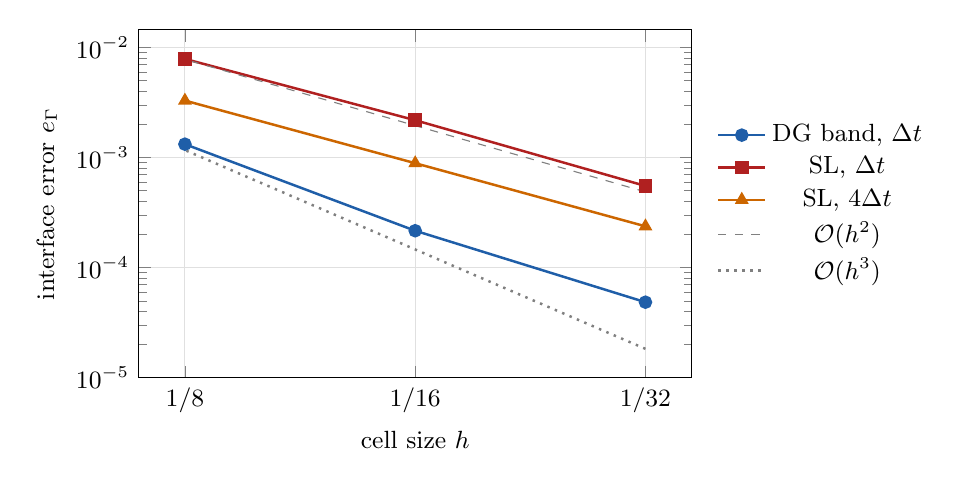
\begin{tikzpicture}
    \begin{loglogaxis}[
        width=8.6cm, height=6.0cm,
        xlabel={cell size $h$}, ylabel={interface error $e_\Gamma$},
        x dir=reverse,
        xtick={0.125,0.0625,0.03125}, xticklabels={$1/8$,$1/16$,$1/32$},
        legend style={font=\small, at={(1.03,0.5)}, anchor=west, draw=none},
        tick label style={font=\small}, label style={font=\small},
        grid=major, grid style={black!12}]
      \addplot[mark=*, accent, line width=0.9pt] coordinates
        {(0.125,1.3244e-3) (0.0625,2.1656e-4) (0.03125,4.8573e-5)};
      \addlegendentry{DG band, $\Delta t$}
      \addplot[mark=square*, ifcol, line width=0.9pt] coordinates
        {(0.125,7.8813e-3) (0.0625,2.1865e-3) (0.03125,5.5279e-4)};
      \addlegendentry{SL, $\Delta t$}
      \addplot[mark=triangle*, orange!80!black, line width=0.9pt] coordinates
        {(0.125,3.2968e-3) (0.0625,8.8953e-4) (0.03125,2.3752e-4)};
      \addlegendentry{SL, $4\Delta t$}
      \addplot[black!50, dashed, domain=0.03125:0.125] {0.5*x^2};
      \addlegendentry{$\mathcal{O}(h^2)$}
      \addplot[black!50, dotted, line width=0.9pt, domain=0.03125:0.125] {0.6*x^3};
      \addlegendentry{$\mathcal{O}(h^3)$}
    \end{loglogaxis}
  \end{tikzpicture}
  \caption{Rotating circle: convergence of the interface error. The semi-Lagrangian method converges
  with second order; the larger time step reduces the error by a factor of about 2.4.}
  \label{fig:rc}
\end{figure}

\paragraph{Single vortex.}
A circle of radius $0.15$ centered at $(0.5, 0.75)$ in $\Omega = [0,1]^2$ is stretched by the
time-reversed vortex $\uu = \cos(\pi t/T)\,\big(\sin(2\pi y)\sin^2(\pi x),
-\sin(2\pi x)\sin^2(\pi y)\big)$ (LeVeque~\cite{LeVeque1996}) and returns to its initial shape at
$t = T$. Table~\ref{tab:vortex} lists the results; the area error is the relative change of the
enclosed area between $t = 0$ and $t = T$, and the circularity is $2\sqrt{\pi A}/|\Gamma_h|$.

\begin{table}[ht]
  \centering
  \small
  \caption{Single vortex at $t = T$ ($f$: reinitialization frequency). DG band: ghost-penalty
  extension.}
  \label{tab:vortex}
  \begin{tabular}{@{}llcccrrr@{}}
    \toprule
    method & cells & $T$ & $\Delta t$ & $f$ & $e_\Gamma$ & area error & circularity \\
    \midrule
    DG band & $32^2$ & 2 & 0.002 & 10 & \multicolumn{3}{c}{fails at $t \approx 1.22$ (spurious interfaces)} \\
    DG band & $64^2$ & 2 & 0.001 & 10 & $1.58\cdot10^{-4}$ & $-0.06\,\%$ & 1.000 \\
    SL      & $32^2$ & 2 & 0.01  & 2  & $1.56\cdot10^{-3}$ & $+0.10\,\%$ & 0.998 \\
    SL      & $32^2$ & 2 & 0.002 & 10 & \multicolumn{3}{c}{degrades after $t \approx 1.6$} \\
    SL      & $64^2$ & 2 & 0.005 & 2  & $2.25\cdot10^{-4}$ & $-0.02\,\%$ & 1.000 \\
    SL      & $32^2$ & 4 & 0.01  & 2  & $1.31\cdot10^{-2}$ & $-1.1\,\%$  & 0.91 \\
    SL      & $64^2$ & 4 & 0.005 & 2  & $5.59\cdot10^{-2}$ & $+0.75\,\%$ & 0.69 \\
    \bottomrule
  \end{tabular}
\end{table}

For $T = 4$, the tail of the spiral becomes thinner than a cell at both resolutions
(Figure~\ref{fig:vortex}). With the semi-Lagrangian method, the under-resolved tail breaks into
pieces ($32^2$) or pinches off as a droplet ($64^2$), which does not merge back; this droplet
dominates the interface error and the circularity at $64^2$. No spurious interfaces appear, and the
number of cut cells stays bounded. On the coarse mesh the result is sensitive to small
perturbations: with 4 instead of 2 MPI processes (different ILU preconditioner of the
reinitialization), the area error at $T = 4$ is $-6\,\%$ instead of $-1.1\,\%$.

\begin{figure}[ht]
  \centering
  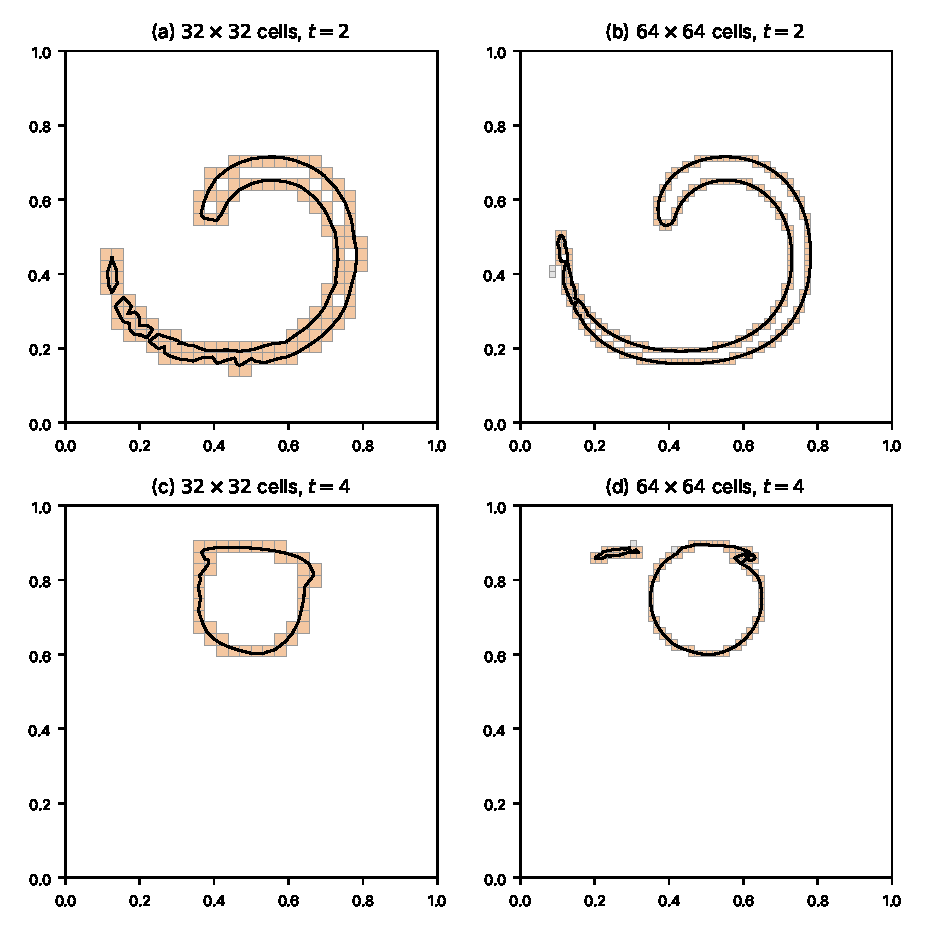
\includegraphics[width=0.68\textwidth]{vortex_T4.pdf}
  \caption{Single vortex with $T = 4$, semi-Lagrangian narrow band: cut cells (orange) and zero level
  set at maximum stretching ($t = 2$) and at the end ($t = 4$).}
  \label{fig:vortex}
\end{figure}

\FloatBarrier
\section{Parameters and limitations}
\label{sec:params}

\begin{table}[H]
  \centering
  \small
  \caption{Recommended parameters of the semi-Lagrangian narrow band.}
  \label{tab:params}
  \begin{tabular}{@{}ll@{}}
    \toprule
    parameter & value \\
    \midrule
    \texttt{narrow band/type} & \texttt{semi\_lagrangian} \\
    \texttt{time stepping/time step size} & max.\ displacement$/h \approx 0.3$--$0.7$ \\
    \texttt{narrow band/reinitialization frequency} & 2 \\
    \texttt{reinitialization/type} & \texttt{elliptic} \\
    \texttt{reinitialization/elliptic/intersected cells only} & \texttt{true} \\
    \texttt{reinitialization/elliptic/penalty parameter} & $10^4$ \\
    \bottomrule
  \end{tabular}
\end{table}

\begin{itemize}
  \item The displacement per step must stay below one cell; foot points outside the vertex
  neighborhood are reported as \emph{not located} and get the sign of the Taylor value.
  \item Small time steps accumulate interpolation errors. When coupled to a flow solver with small
  time steps, the level set should be advected only every $k$-th flow step.
  \item The velocity is evaluated at arbitrary points and intermediate times. With a discrete velocity
  field, this requires point evaluation across processes and interpolation in time.
  \item All cut cells are gathered on every process for the closest-point search. This is acceptable
  for 2D and moderate 3D interfaces; large 3D runs need a local search among neighboring processes.
  \item The implementation requires parallelepiped cells, tensor-product nodal elements
  (\texttt{FE\_DGQ}) and meshes without hanging nodes. The method is not conservative.
\end{itemize}

\begin{thebibliography}{9}
\bibitem{Adams2019}
T.~Adams, S.~Giani, W.~M.~Coombs.
A high-order elliptic PDE based level set reinitialisation method using a discontinuous Galerkin
discretisation.
\emph{Journal of Computational Physics} 379 (2019) 373--391.

\bibitem{BastingKuzmin2013}
C.~Basting, D.~Kuzmin.
A minimization-based finite element formulation for interface-preserving level set
reinitialization.
\emph{Computing} 95 (2013) S13--S25.

\bibitem{LeVeque1996}
R.~J.~LeVeque.
High-resolution conservative algorithms for advection in incompressible flow.
\emph{SIAM Journal on Numerical Analysis} 33(2) (1996) 627--665.

\bibitem{Saye2014}
R.~I.~Saye.
High-order methods for computing distances to implicitly defined surfaces.
\emph{Communications in Applied Mathematics and Computational Science} 9(1) (2014) 107--141.

\bibitem{Saye2015}
R.~I.~Saye.
High-order quadrature methods for implicitly defined surfaces and volumes in hyperrectangles.
\emph{SIAM Journal on Scientific Computing} 37(2) (2015) A993--A1019.
\end{thebibliography}

\end{document}
